\subsection{Chord of a Circle}

\begin{figure}[!h]
	\begin{center}
		
		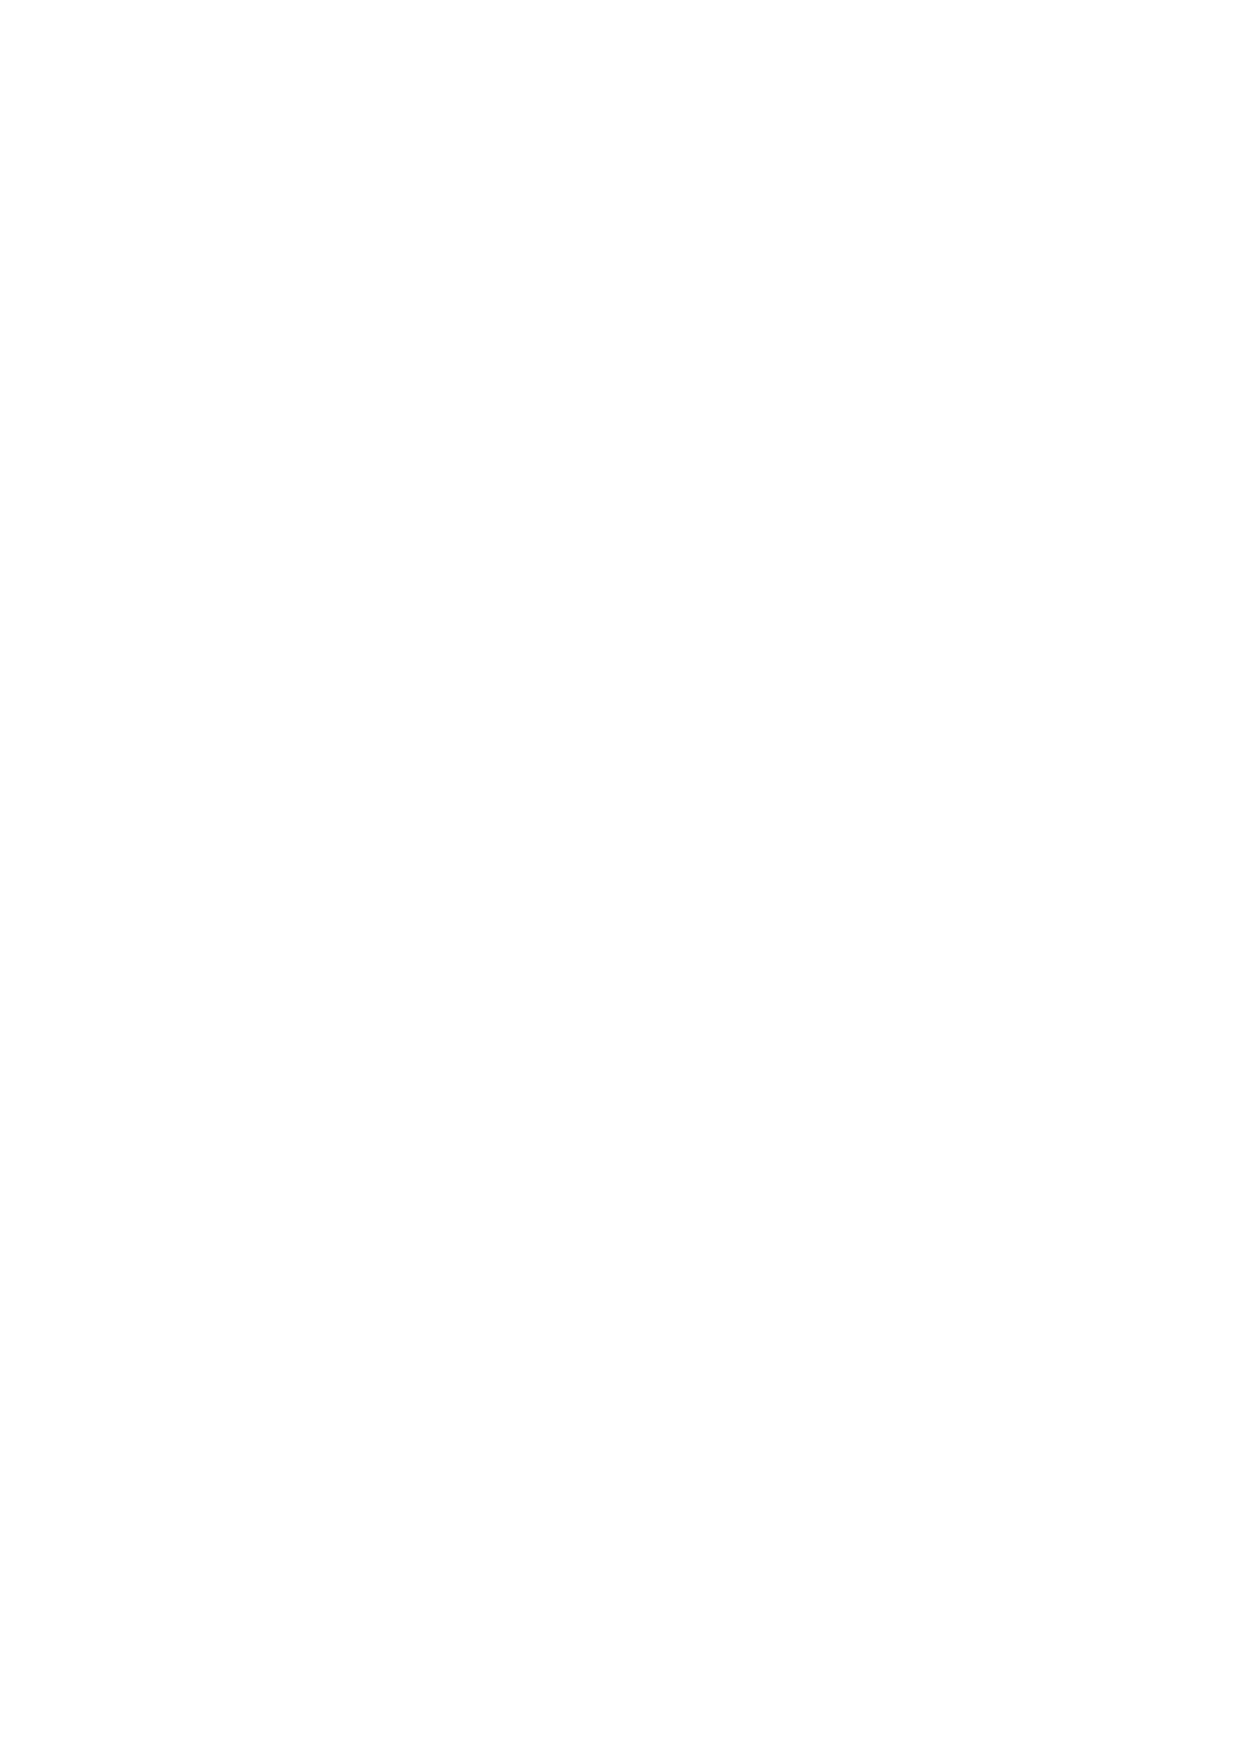
\includegraphics[width=\columnwidth]{./figs/ch4_circle_def}
		\vspace*{-10cm}
	\end{center}
	\caption{Circle Definitions}
	\label{ch4_circle_def}	
\end{figure}
\begin{definition}
	Fig. \ref{ch4_circle_def} represents a circle.  The points in the circle are at a distance $r$ from the centre $O$.  $r$ is known as the radius.
\end{definition}

\subsection{Chords of a circle}
\begin{definition}
	In Fig. \ref{ch4_circle_def}, $A$ and $B$ are points on the circle.  The line $AB$ is known as a chord of the circle.
\end{definition}
%
%
\begin{problem}
	\label{ch4_prob_circle_subtend}
	In Fig. \ref{ch4_circle_subtend}  Show that $\angle OAB = 2\angle APB $.
\end{problem}
\begin{figure}[!h]
	\begin{center}
		
		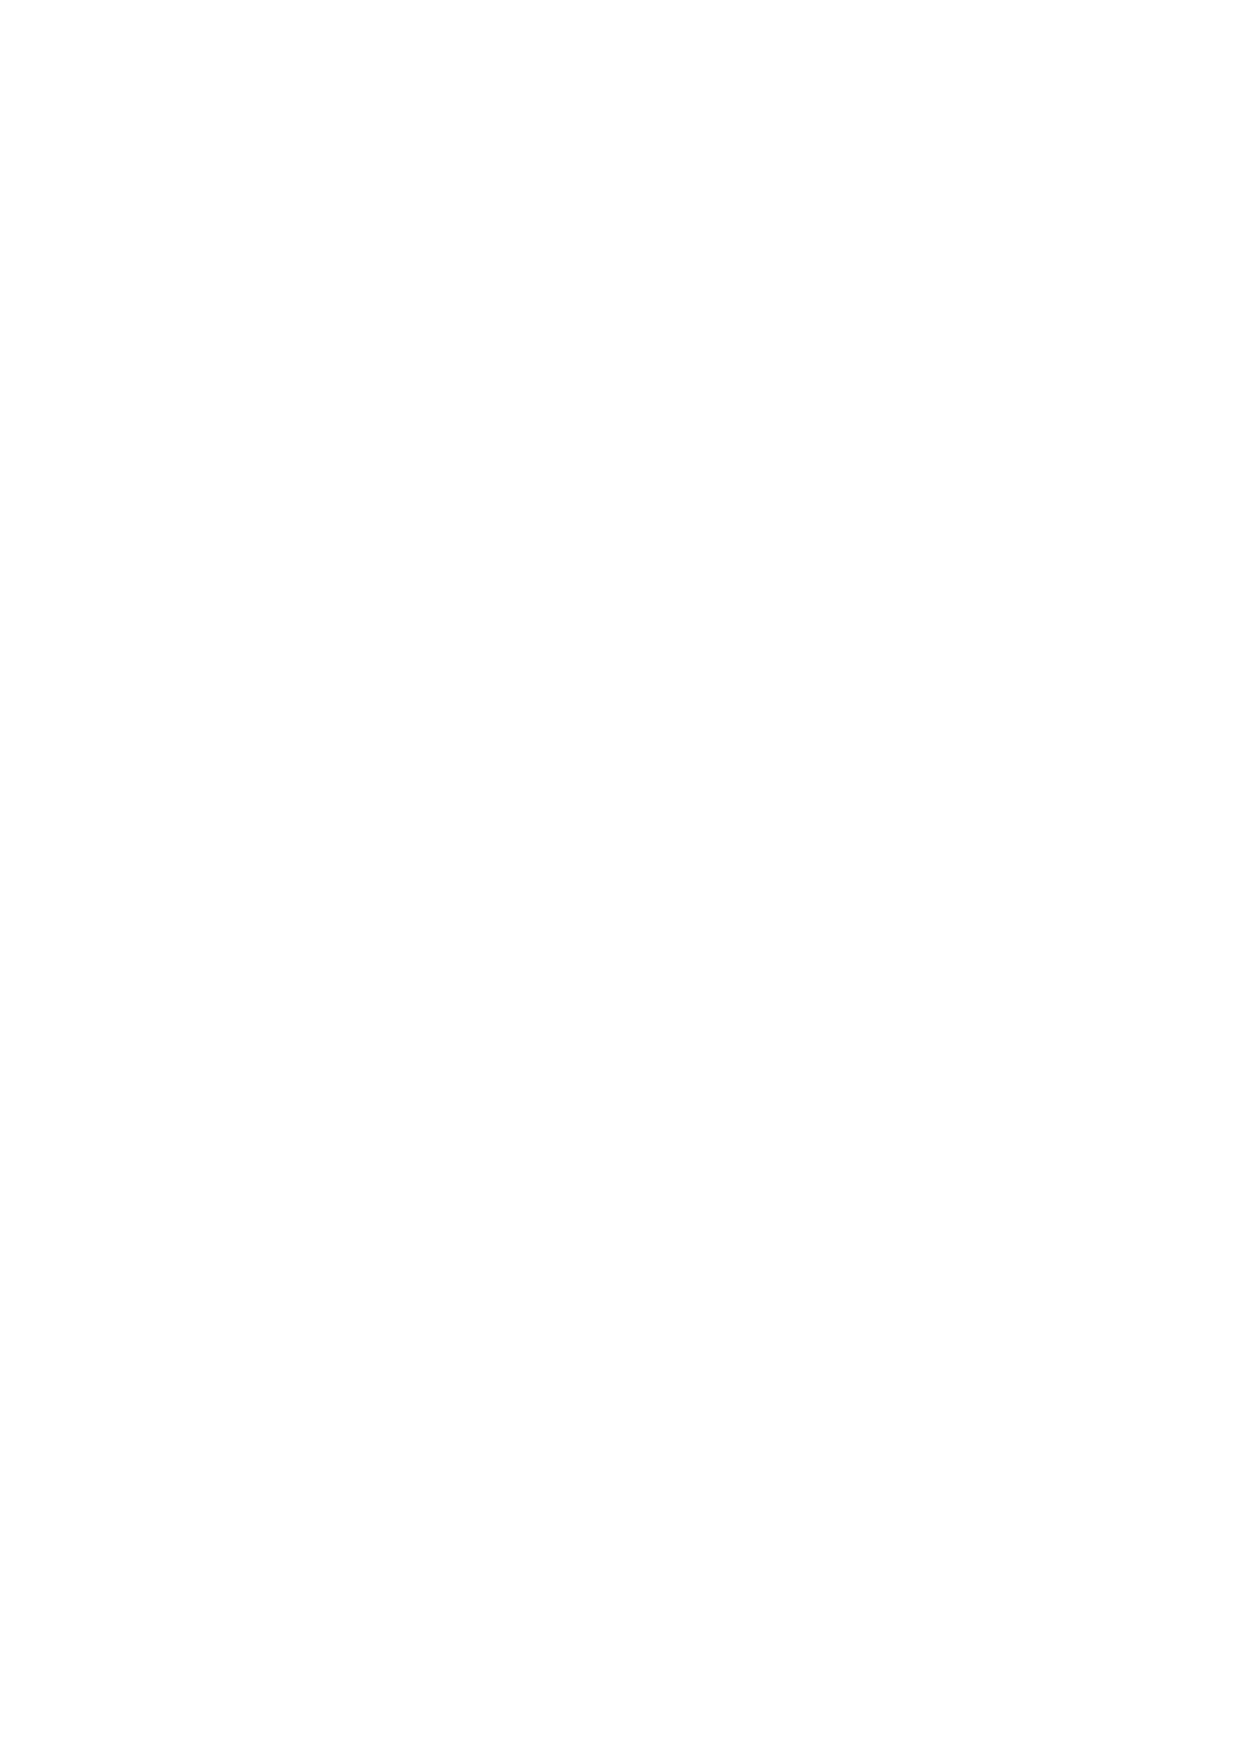
\includegraphics[width=\columnwidth]{./figs/ch4_circle_subtend}
		\vspace*{-10cm}
	\end{center}
	\caption{Angle subtended by chord $AB$ at the centre $O$ is twice the angle subtended at $P$. }
	\label{ch4_circle_subtend}	
\end{figure}

\proof In Fig. \ref{ch4_circle_subtend}, the triangeles $OPA$ and $OPB$ are isosceles. Hence,
%
\begin{align}
\angle OPB = \angle OBP &= \theta_1 \\
\angle OPA = \angle OAP &= \theta_2
\end{align}
%
Also, $\alpha$ and $\beta$ are exterior angles corresponding to the triangle $OPB$ and $OPA$ respectively. Hence
%
\begin{align}
\alpha &= 2\theta_1 \\
\beta &= 2\theta_2
\end{align}
%
Thus,
%
\begin{align}
\angle AOB &= \alpha + \beta \\
&= \theta_1 + \theta_2 \\
&= \angle APB
\end{align}
%
\begin{definition}
	The diameter of a circle is the chord that divides the circle into two equal parts. In Fig. \ref{ch4_circle_dia}, $AB$ is the diameter and passes through the centre $O$
\end{definition}
%
\begin{problem}
In Fig. \ref{ch4_circle_dia}, show that $\angle APB = 90^{\degree}$ .
\end{problem}
%
\begin{figure}[!h]
	\begin{center}
		
		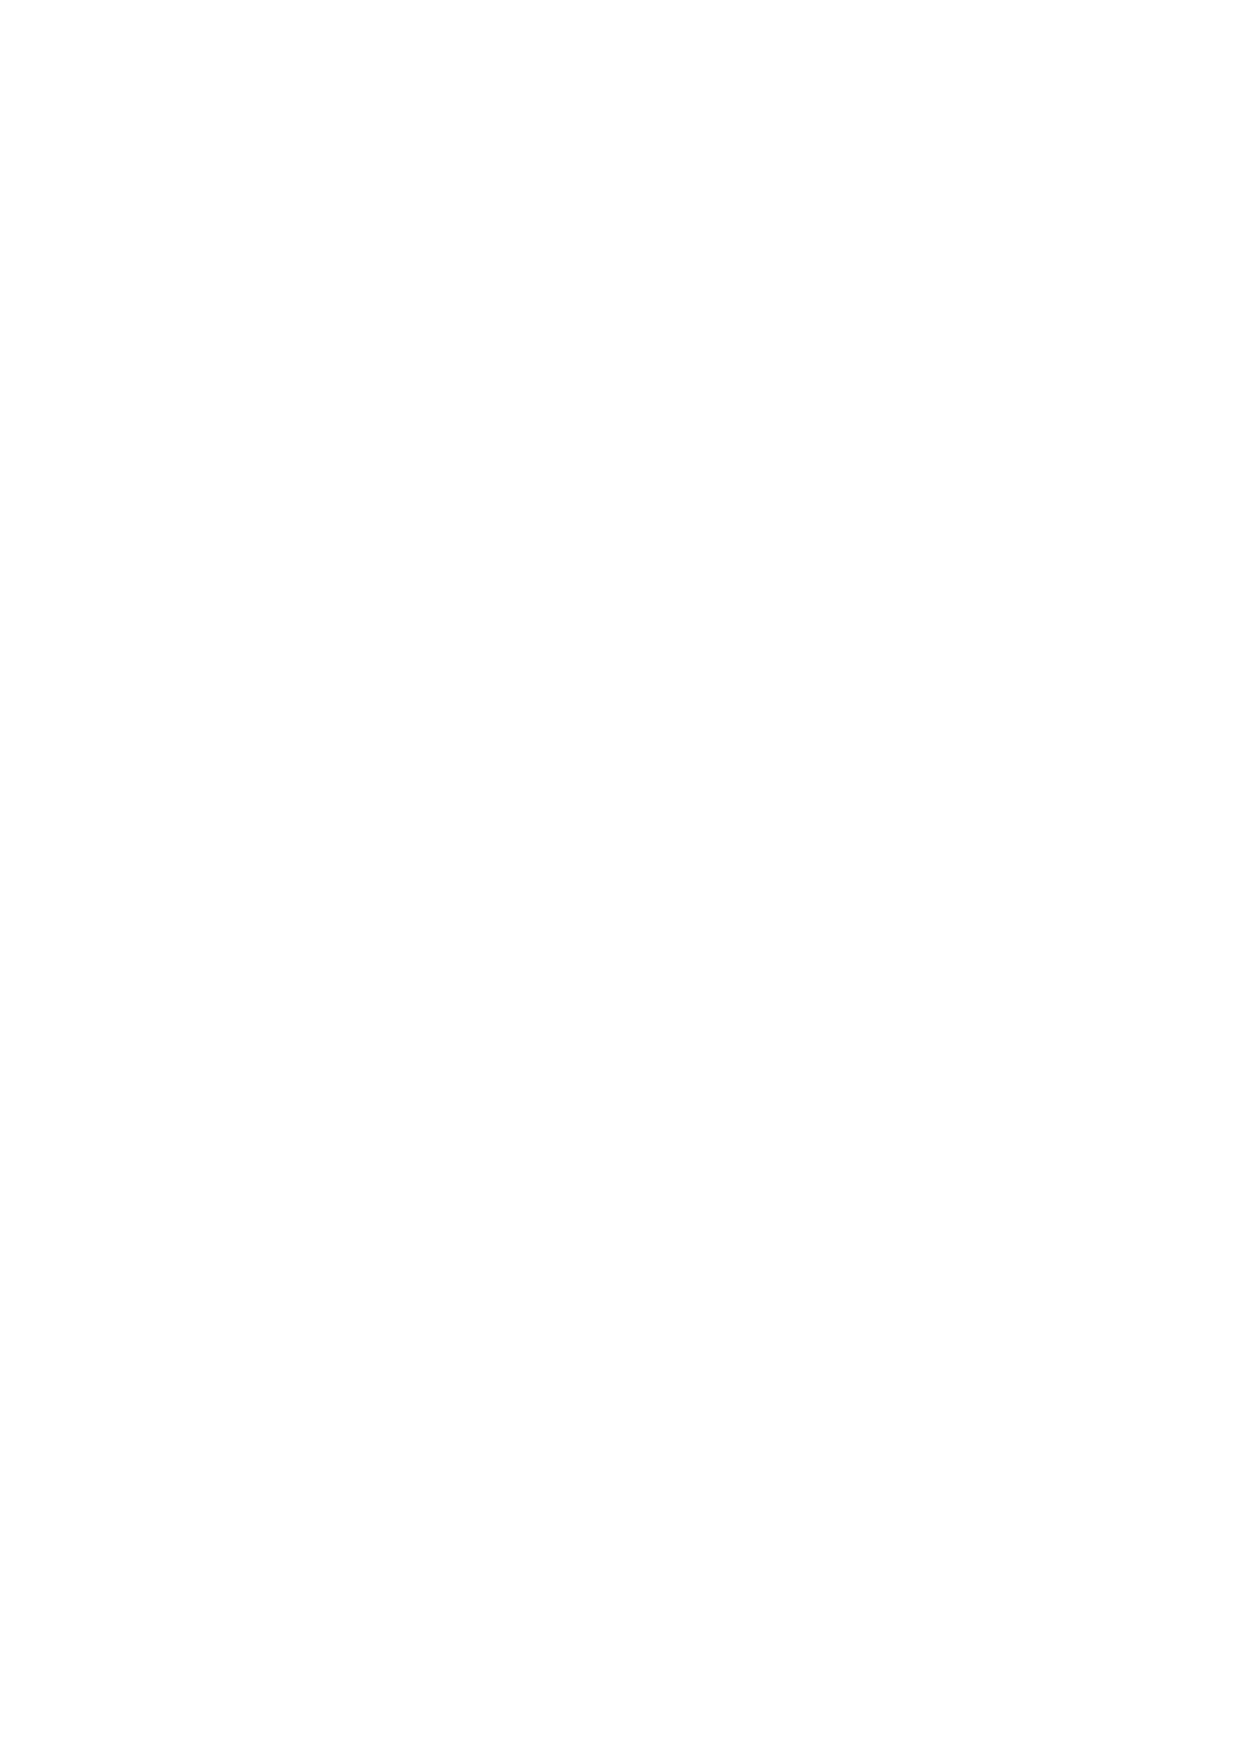
\includegraphics[width=\columnwidth]{./figs/ch4_circle_dia}
		\vspace*{-10cm}
	\end{center}
	\caption{Diameter of a circle.}
	\label{ch4_circle_dia}	
\end{figure}

\begin{problem}
	In Fig. \ref{ch4_chord_product}, show that 
	\begin{equation}
	\begin{split}
\angle ABD &= \angle ACD \\
\angle CAB &= \angle CDB	
	\end{split}
	\end{equation}
\end{problem}
\begin{figure}[!h]
	\begin{center}
		
		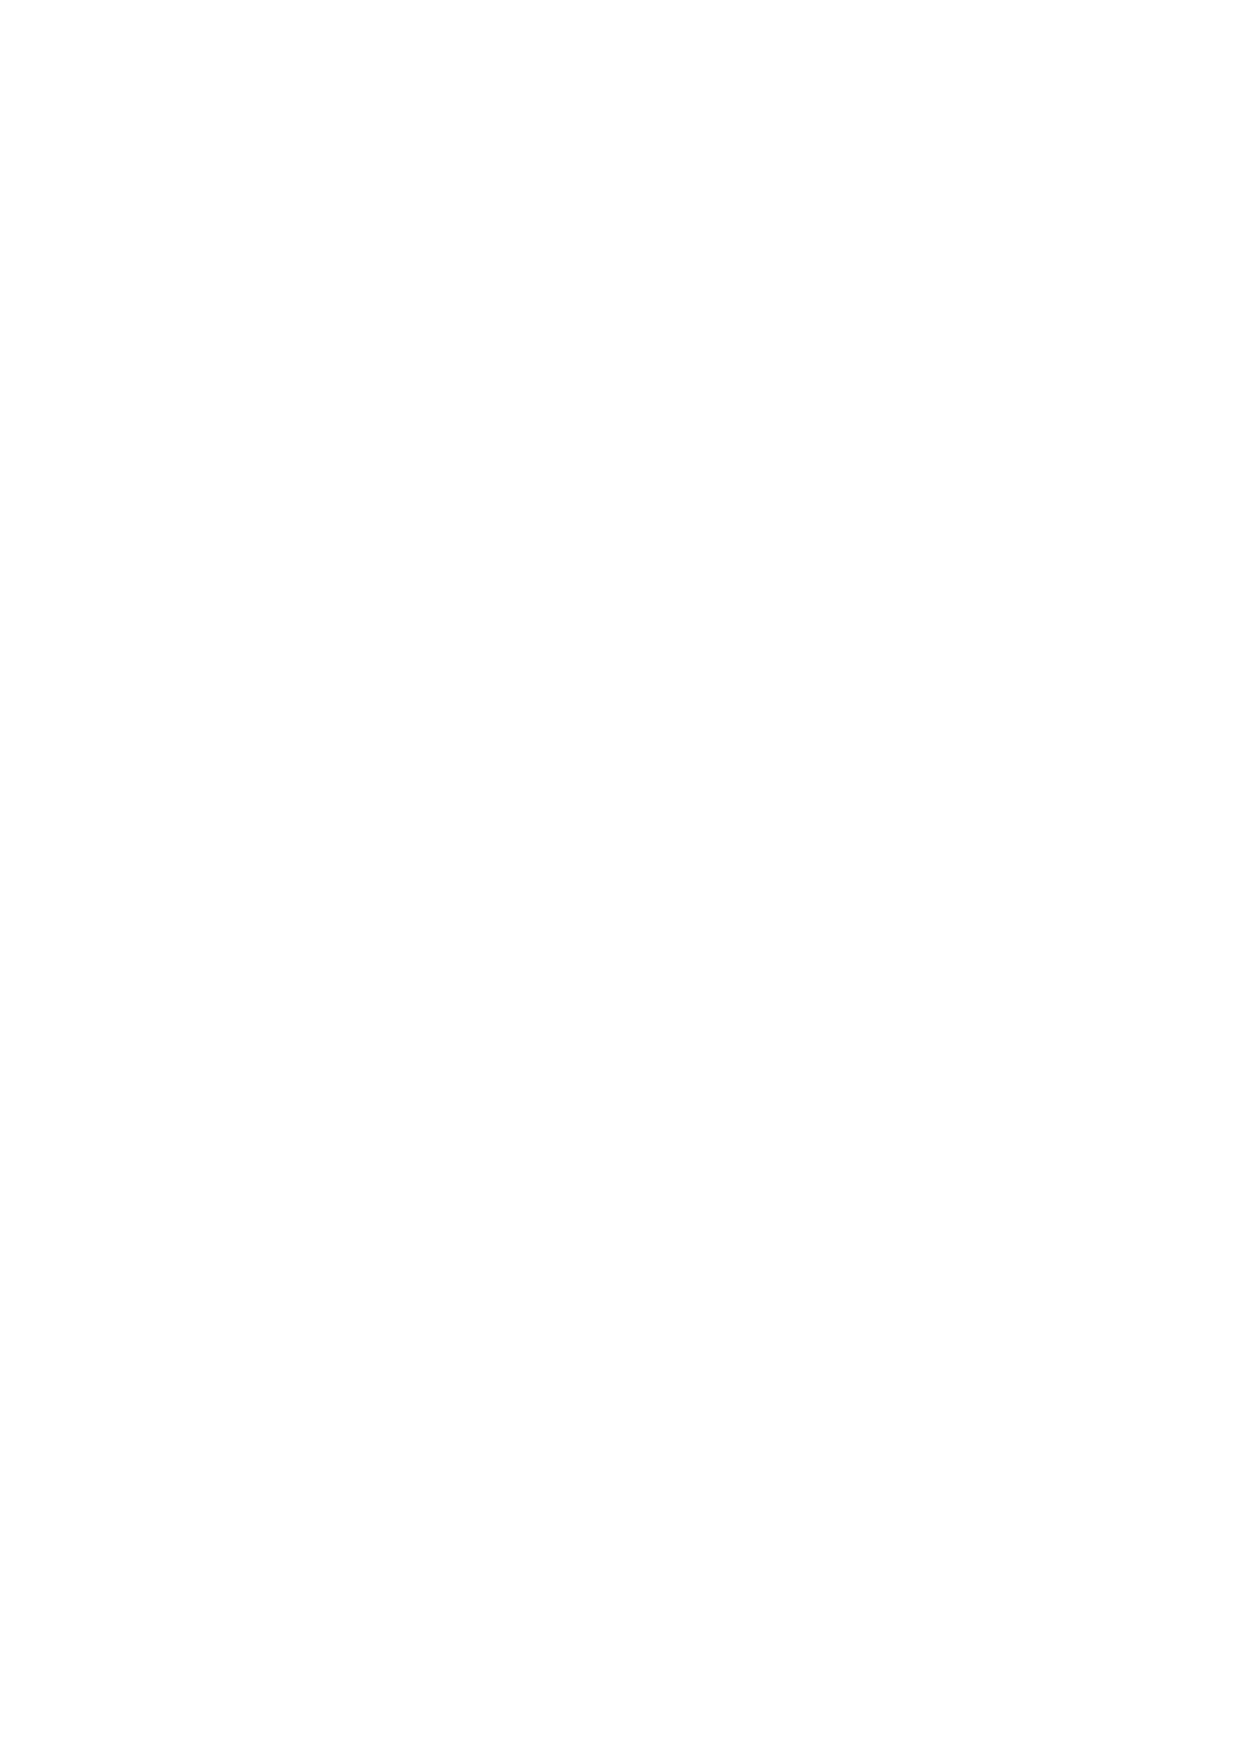
\includegraphics[width=\columnwidth]{./figs/ch4_chord_product}
		\vspace*{-10cm}
	\end{center}
	\caption{$PA.PB = PC.PD$}
	\label{ch4_chord_product}	
\end{figure}
%
%
\proof Use Problem \ref{ch4_prob_circle_subtend}.
%
\begin{problem}
	In Fig. \ref{ch4_chord_product}, show that the triangles $PAB$ and $PBD$ are similar
\end{problem}
\proof Trivial using previous problem
\begin{problem}
	In Fig. \ref{ch4_chord_product}, show that 
	\begin{equation}
	PA.PB = PC.PD
	\end{equation}
\end{problem}
%
\proof Since triangles $PAC$ and $PBD$ are similar, 
%
\begin{align}
\frac{PA}{PD} &= \frac{PC}{PB} \\
\Rightarrow PA.PB &= PC.PD
\end{align}
%
%
\begin{definition}
	The line $PX$ in Fig. \ref{ch4_tangent_def} touches the circle at exactly one  point $P$. It is known as the tangent to the circle.
\end{definition}
%
%
\begin{problem}
	$OP$ is the perpendicular to the line $PX$ as shown in the Fig. \ref{ch4_short_dist}. Show that $OP$ is the shortest distance between the point $O$ and the line $PX$. 
\end{problem}
\proof Let $P_1$ be a point on the line $PX$. Then $OPP_1$ is a right angled triangle.  Using Budhayana's theorem,
%
\begin{figure}[!h]
	\begin{center}
		
		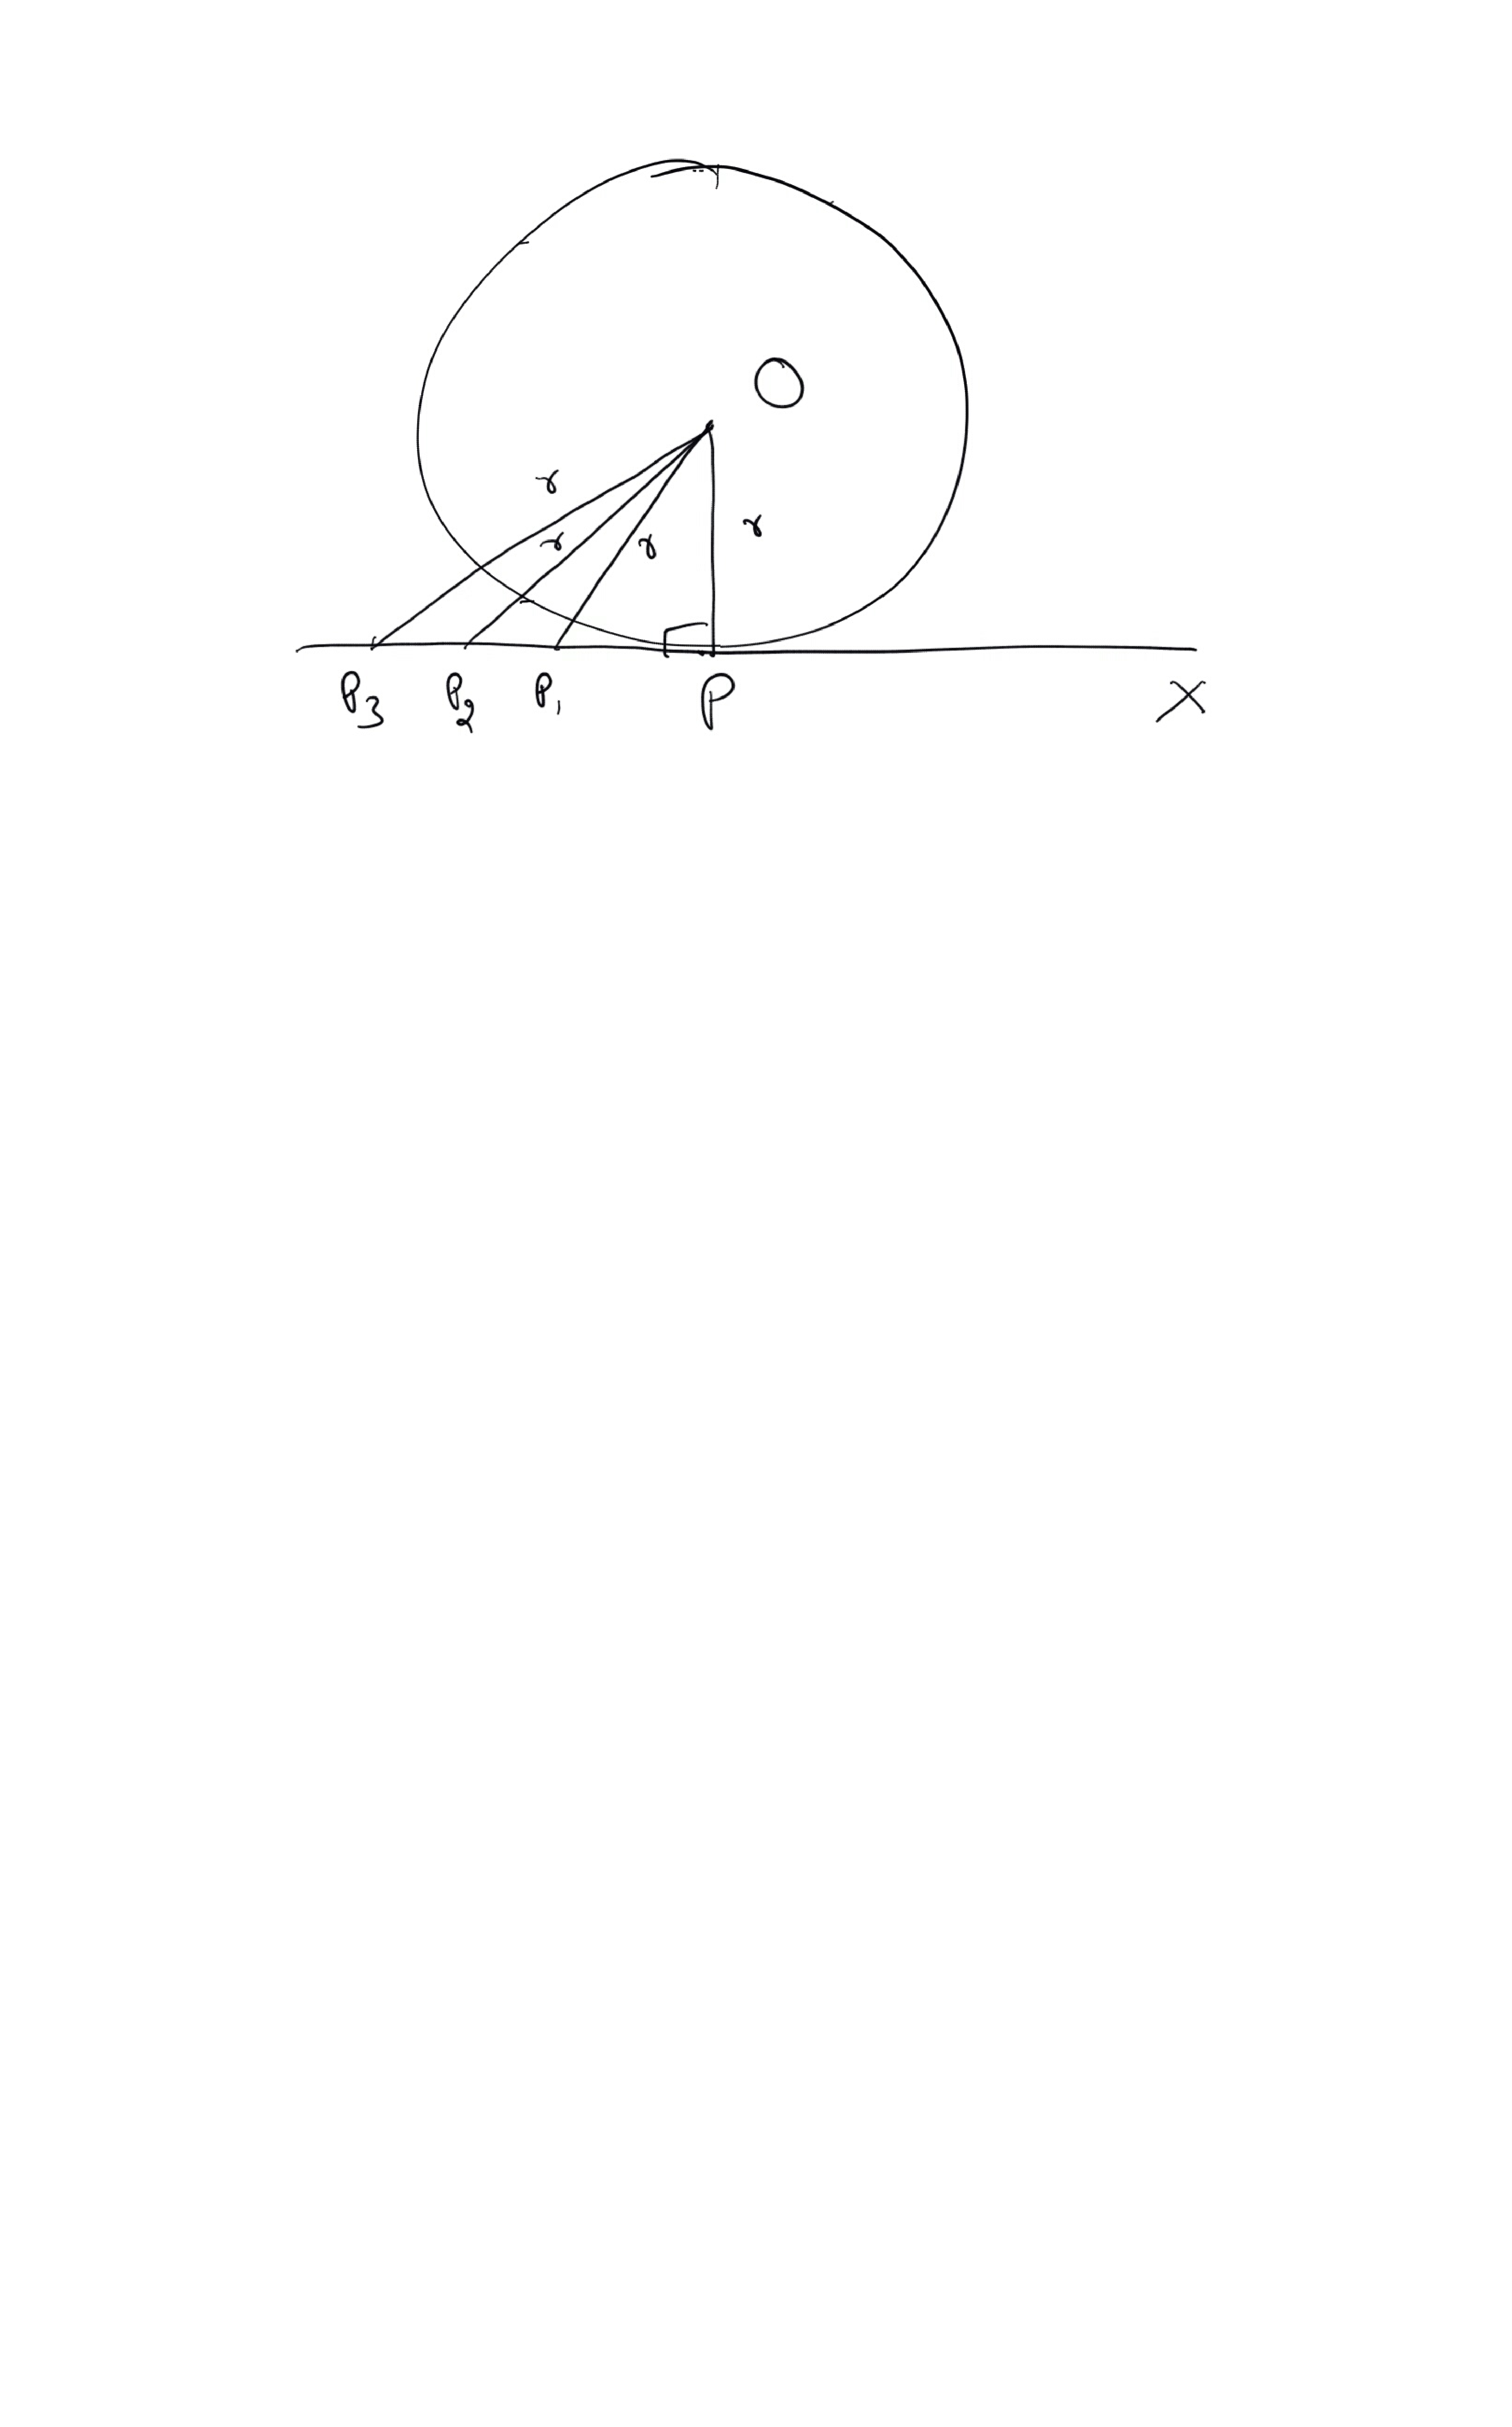
\includegraphics[width=\columnwidth]{./figs/ch4_tangent_def}
		\vspace*{-10cm}
	\end{center}
	\caption{Tangent to a Circle.}
	\label{ch4_tangent_def}	
\end{figure}
%
\begin{figure}[!h]
	\begin{center}
		
		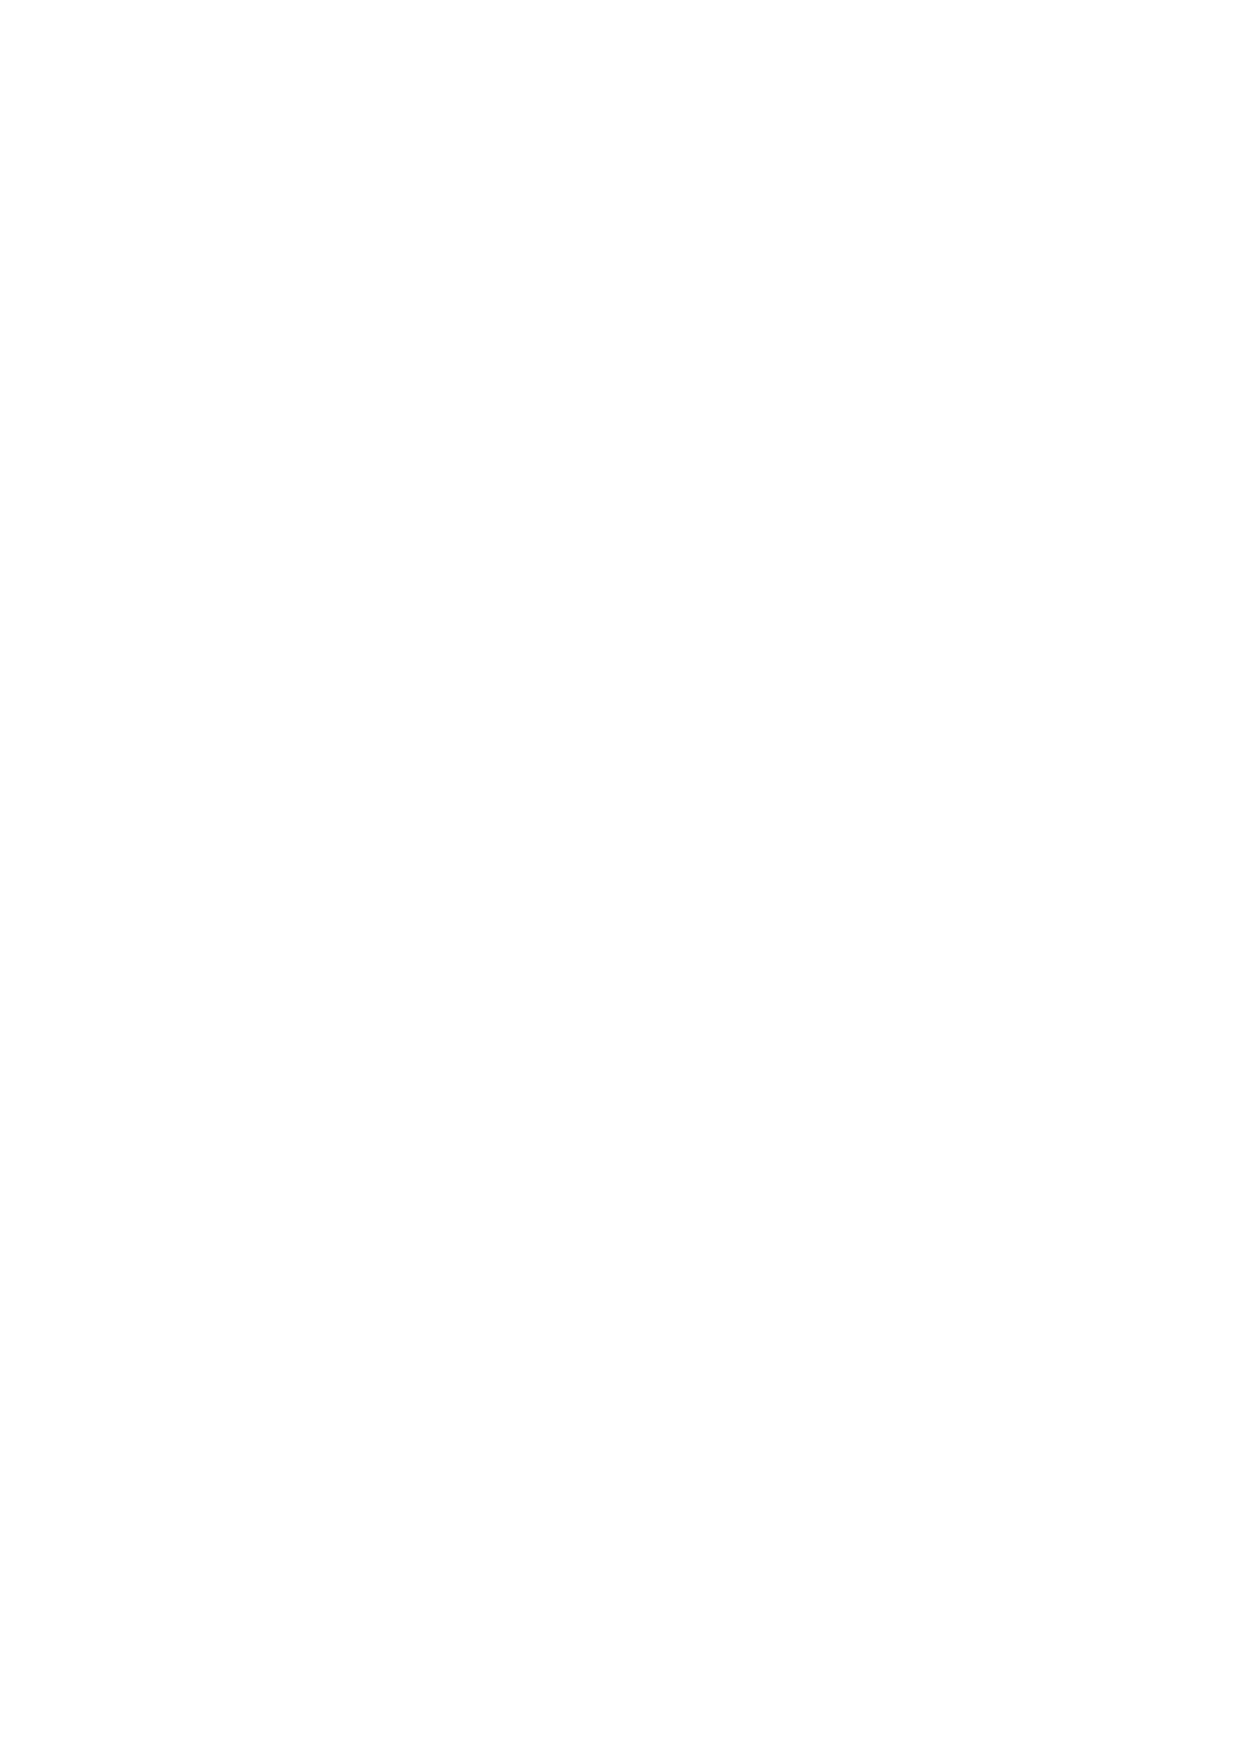
\includegraphics[width=\columnwidth]{./figs/ch4_short_dist}
		\vspace*{-10cm}
	\end{center}
	\caption{Shortest distance from $O$ to line $PX$}
	\label{ch4_short_dist}	
\end{figure}

%
\begin{equation}
\begin{split}
OP_1^2 &= OP^2 + PP_1^2 \\
\Rightarrow OP_1 > OP
\end{split}
\end{equation}
%
Thus, $OP$ is the shortest distance between $O$ and line $PX$.
%
\begin{problem}
Show that $\angle OPX = 90 ^{\degree}$
\end{problem}
\proof In Fig. \ref{ch4_tangent_def}, we can see that $OP$ is is the radius of the circle and the length of all line segments from $O$ to the line $PX > r$.  Using the result of the previous 
problem, it is obvious that $OP \perp PX$. 
%
	%
\begin{problem}
In Fig. \ref{ch4_tangent_prod} show that 
%
\begin{equation}
\angle PCA = \angle PBC
\end{equation}
%
$O$ is the centre of the circle and $PC$ is the tangent.
\end{problem}
	\begin{figure}[!h]
		\begin{center}
			
			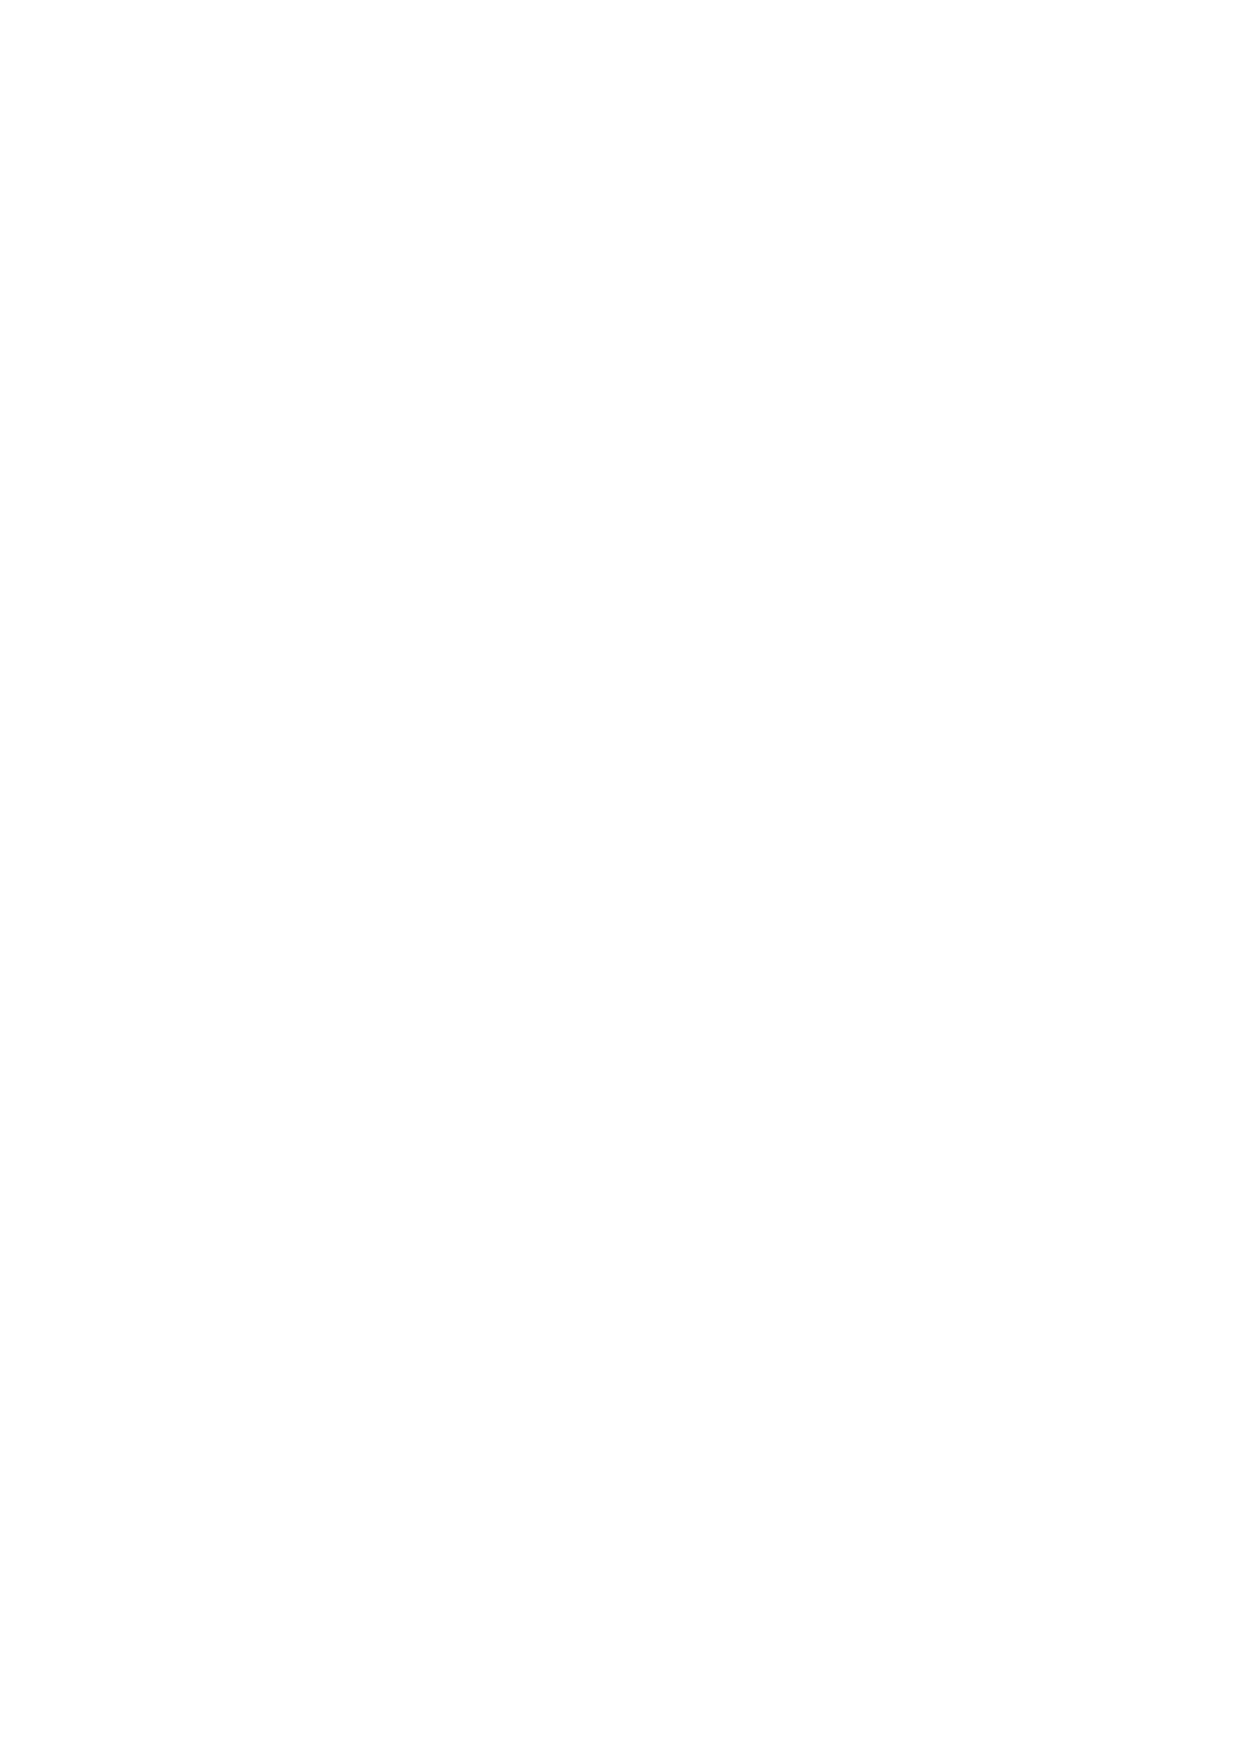
\includegraphics[width=\columnwidth]{./figs/ch4_tangent_prod}
			\vspace*{-10cm}
		\end{center}
		\caption{$PA.PB = PC^2$.}
		\label{ch4_tangent_prod}	
	\end{figure}
	%

%
\proof For convenience, greek letters are used for representing certain angles. Since $\Delta OAC$ is isosceles,
%
\begin{align}
2 \alpha + 2 \brak{\beta - \phi} &= 180^{\degree} \\
\Rightarrow  \alpha +  \brak{\beta - \phi} &= 90^{\degree} \\
\Rightarrow  \alpha +  \beta  &= 90^{\degree} + \phi
\end{align}
%
Since $theta$ is an exterior angle for the $\Delta ABC
$,
%
\begin{equation}
\theta = \alpha + \beta
\end{equation}
%
From both the above equations
%
\begin{equation}
\theta = 90^{\degree} + \phi
\end{equation}
%
Since PC is the tangent, 
%
\begin{equation}
\angle PCB = 90^{\degree} + \phi = \theta
\end{equation}
%
Considering the sum of angles in $\Delta PAC$ $\Delta PBC$,
%
\begin{align}
\angle P + \theta + \angle PCA &= 180^{\degree} \\
\angle P + \theta + \alpha &= 180^{\degree}
\end{align}
Hence,
%
\begin{equation}
\angle PCA = \alpha
\end{equation}
%
\begin{problem}
	In Fig. \ref{ch4_tangent_prod}, show that the triangles $PAC$ and $PBC$ are similar.
\end{problem}
\proof From the previous problem, it is obvious that corresponding angles of both triangles are equal.  Hence they are similar.
%
\begin{problem}
	Show that $PA.PB = PC^2$
\end{problem}
\proof Since $\Delta PAC \sim \Delta PBC$, their sides are in the same ratio.  Hence,
%
\begin{align}
\frac{PA}{PC} &= \frac{PC}{PB} \\
\Rightarrow PA.PB &=PC^2
\end{align}
%
%
\begin{problem}
	In Fig. \ref{ch4_chord_tangent_prod}, show that\begin{equation}
	PA.PB = PC.PD
	\end{equation}
\end{problem}
%
\begin{figure}[!h]
	\begin{center}
		
		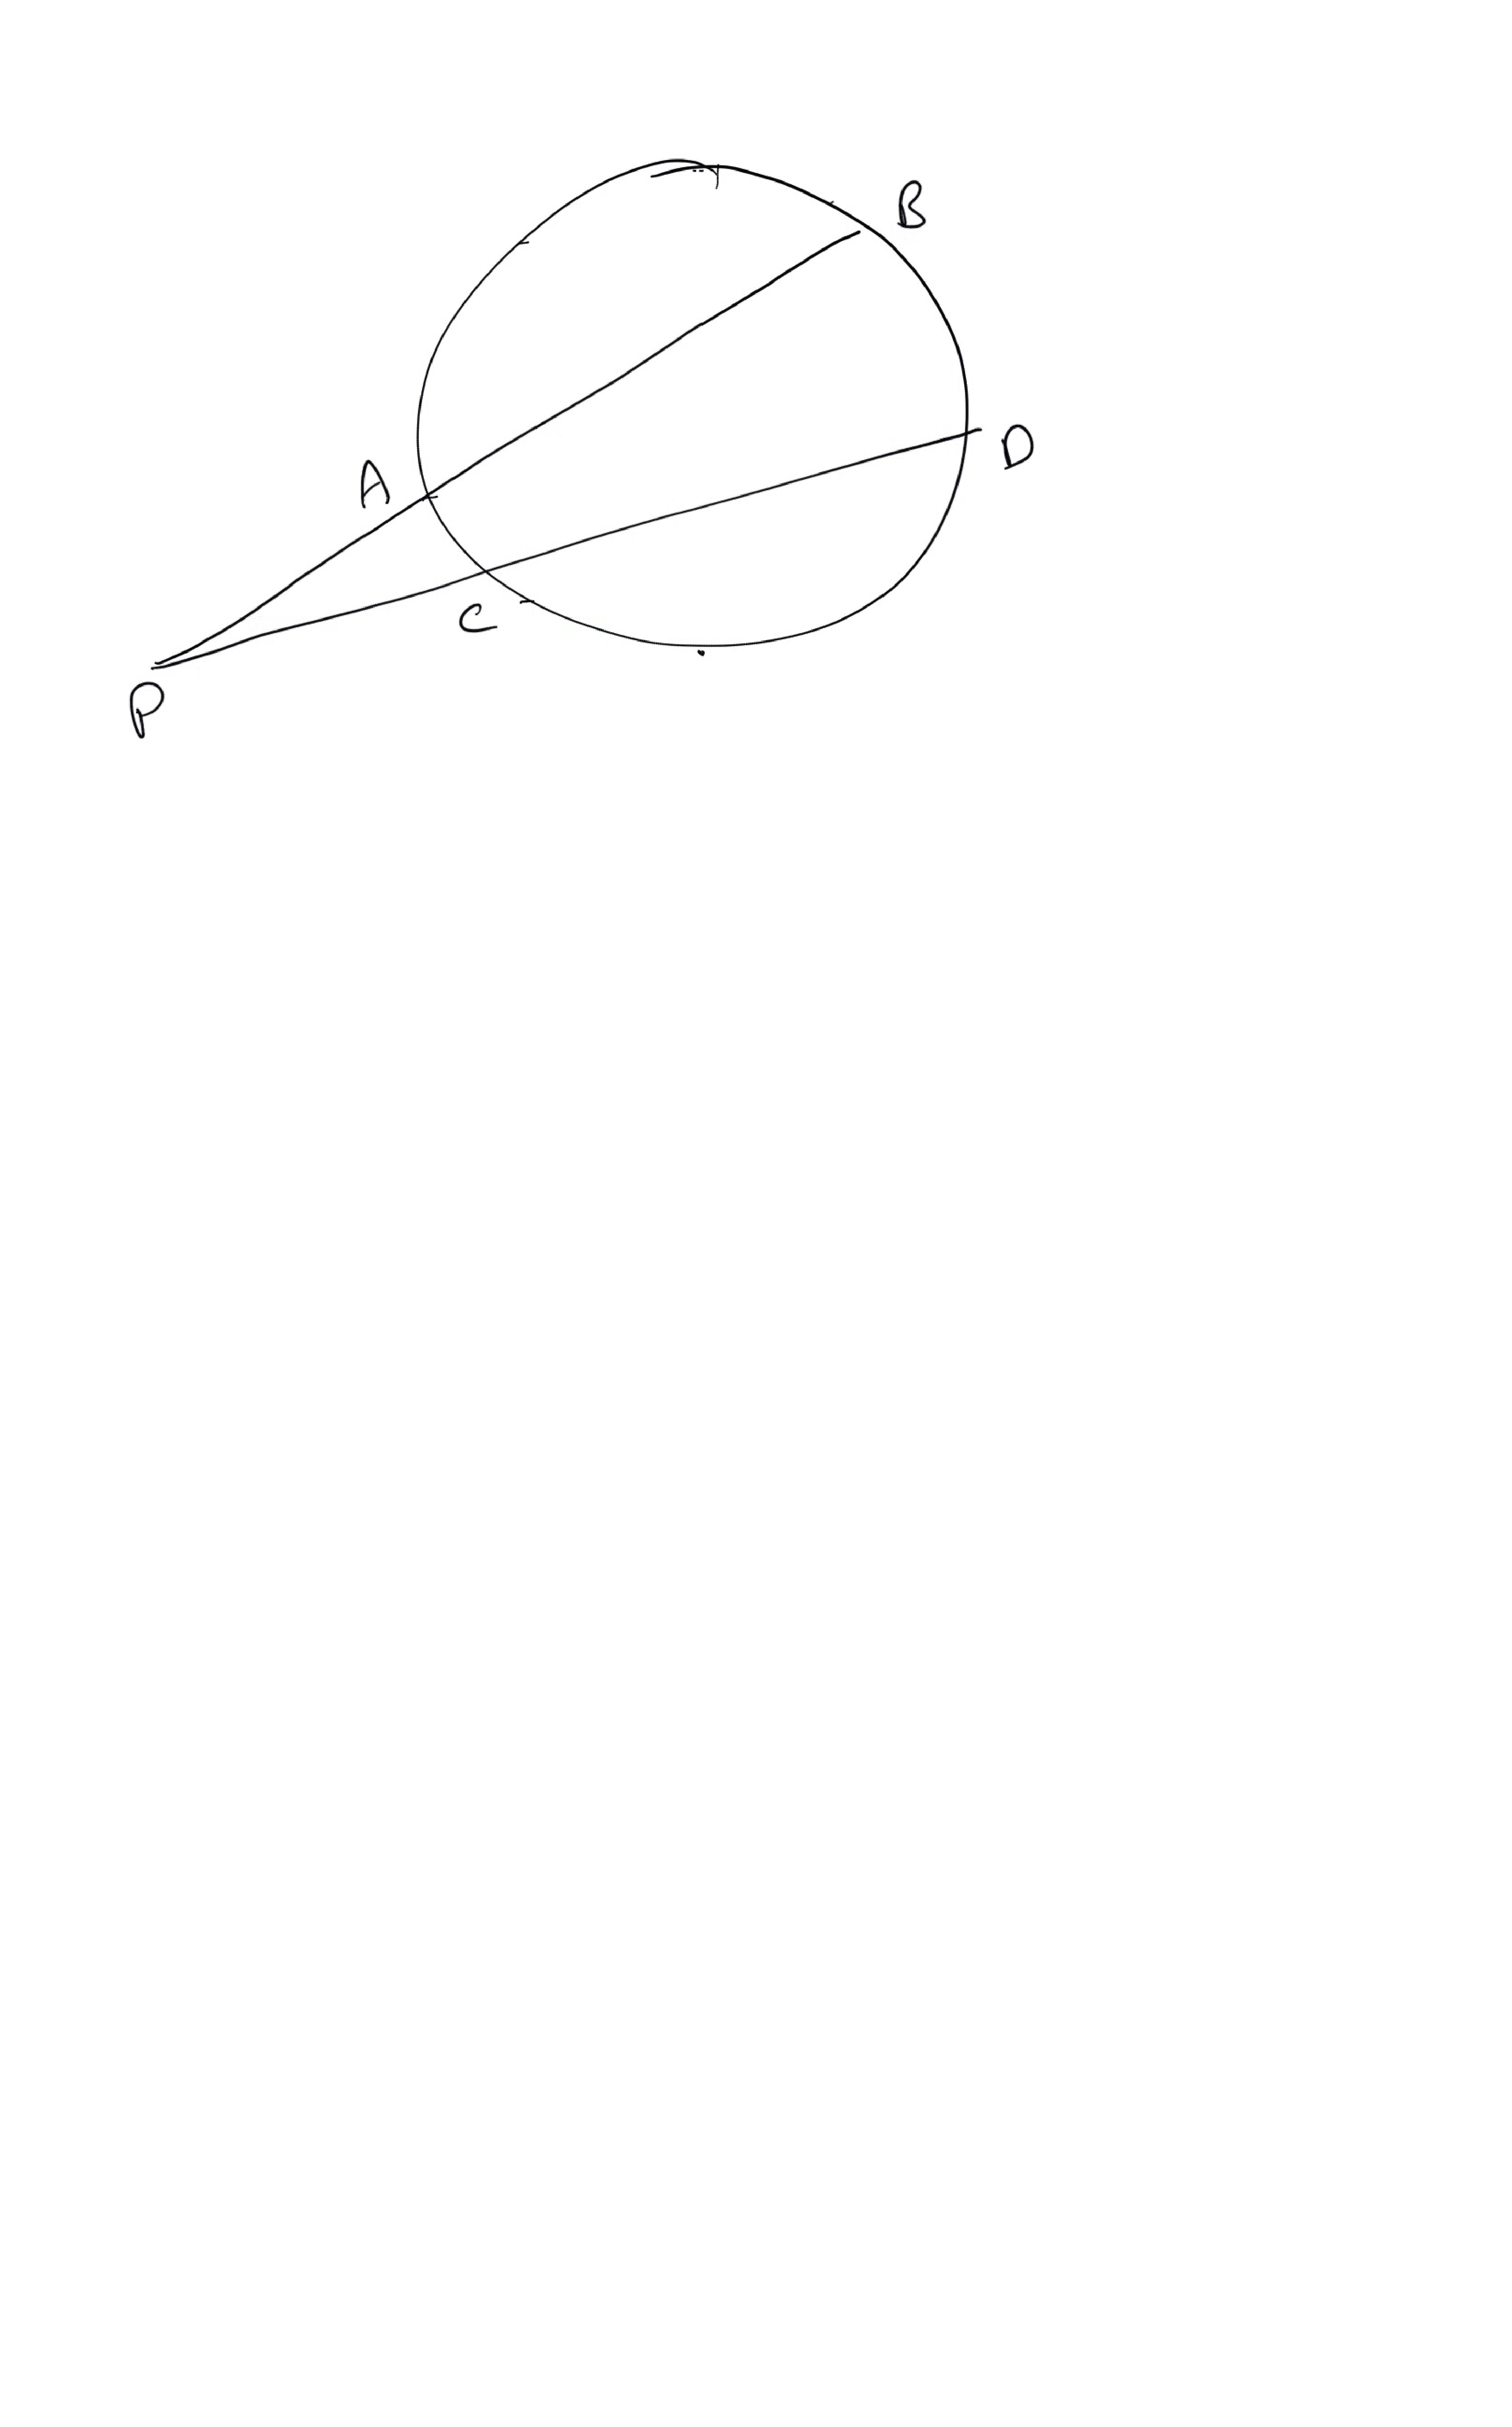
\includegraphics[width=\columnwidth]{./figs/ch4_chord_tangent_prod}
		\vspace*{-10cm}
	\end{center}
	\caption{$PA.PB = PC^2$.}
	\label{ch4_chord_tangent_prod}	
\end{figure}

\proof Draw a tangent and use the previous problem.
